% HW Template for CS 6150, taken from https://www.cs.cmu.edu/~ckingsf/class/02-714/hw-template.tex
%
% You don't need to use LaTeX or this template, but you must turn your homework in as
% a typeset PDF somehow.
%
% How to use:
%    1. Update your information in section "A" below
%    2. Write your answers in section "B" below. Precede answers for all 
%       parts of a question with the command "\question{n}{desc}" where n is
%       the question number and "desc" is a short, one-line description of 
%       the problem. There is no need to restate the problem.
%    3. If a question has multiple parts, precede the answer to part x with the
%       command "\part{x}".
%    4. If a problem asks you to design an algorithm, use the commands
%       \algorithm, \correctness, \runtime to precede your discussion of the 
%       description of the algorithm, its correctness, and its running time, respectively.
%    5. You can include graphics by using the command \includegraphics{FILENAME}
%
\documentclass[11pt]{article}
\usepackage{amsmath,amssymb,amsthm}
\usepackage{graphicx}
\usepackage[margin=1in]{geometry}
\usepackage{fancyhdr}
\usepackage{framed}
\usepackage{algorithm}
\usepackage{algpseudocode}
\usepackage{pifont}
\setlength{\parindent}{0pt}
\setlength{\parskip}{5pt plus 1pt}
\setlength{\headheight}{13.6pt}
\newcommand\question[2]{\vspace{.25in}\hrule\textbf{#1}\vspace{.5em}\hrule\vspace{.10in}}
\renewcommand\part[1]{\vspace{.10in}\textbf{(#1)}}
\newcommand\algorith{\vspace{.10in}\textbf{Algorithm: }}
\newcommand\correctness{\vspace{.10in}\textbf{Correctness: }}
\newcommand\runtime{\vspace{.10in}\textbf{Running time: }}
\pagestyle{fancyplain}
\lhead{\textbf{\NAME\ (\UID)}}
\chead{\textbf{HW\HWNUM}}
\rhead{CS 6490, \today}
\begin{document}\raggedright
%Section A==============Change the values below to match your information==================
\newcommand\NAME{Jake Pitkin}  % your name
\newcommand\UID{u0891770}     % your utah UID
\newcommand\HWNUM{4}              % the homework number
%Section B==============Put your answers to the questions below here=======================

\question{Question 1}

\textbf{Suppose a computer is authenticated based on its IP address (no passwords are used). Identify one strength and one weakness of such an authentication mechanism.}

\textit{Strength:} With an address-based authentication, passwords don't need to be created, remembered, or pass around the network. This makes addressed-based authentication much more convenient than password-based systems. Additionally, passwords can't be intercepted by eavesdroppers, brute force guessed using rainbow tables, or leaked as the result of a compromised database.

\textit{Weakness:} Trudy can impersonate Alice's network address and pose as her on the network. She can perform source routing and inject IP packets to route traffic in such a way that she can transmit from and receive packets for Alice's network address. This comes with it's share of complications (additional cryptographic authentication on the router), as most security threats do.

\question{Question 2}

\part{a} \textbf{Problem 2, Chapter 9, page 236.}

The described scheme guards against eavesdropping but is \textbf{vulnerable to server database disclosure}.

It's secure against eavesdropping as the information Trudy can intercept is: who is trying to authenticate (Alice), a random number R, and the hash of Alice's password and R. Assuming R is sufficiently random and not repeated, $hash(Y,R)$ will not be repeated so this is of no use to Trudy.

However it vulnerable against server database disclosure. Assume Trudy gains access to the database and it contains a table of usernames to hashed passwords for that user. Now Trudy can say to Bob "I'm Alice" and Bob will send Trudy R. Trudy now knows Z (hash of Alice's password) and can compute $hash(Z,R)$ and respond to Bob. Bob will check if this matches $hash(Z,R)$ (which it will) and authenticate Trudy as Alice. 

\part{b} \textbf{Let a dictionary have 4,096 words. Let a user pick 5 words at random for choosing a password (i.e., the password comprises of these 5 words). What is the strength of this password in bits?}

To represent 4,096 words in binary it will require 12-bits. This is because $4,096 = 2^{12}$. As such, each randomly picked word will provide 12-bits of randomness to the password. Since the user chooses 5 words at random, we will concatenate the bit patterns and provide \textbf{60-bit security}.

\question{Question 3}

\part{a} \textbf{Could $\mathbf{f(K_{AB}, R)}$ be a secure hash function of $\mathbf{K_{AB}}$ and R in the protocol below? Explain briefly.}

The protocol is not secure, it is susceptible to an offline dictionary attack by an eavesdropper. 

Trudy can eavesdrop in on Alice and Bob and obtain a set of $f(K_{AB}, R)$ and $R$. Now Trudy can go offline and use brute force to obtain $K_{AB}$. She can generate a guess for Alice and Bob's secret key $K_{G}$ and apply the hash function $f$ to it and $R$. She checks if $f(K_{G}, R) = f(K_{AB}, R)$ and when it does she has found their secret key.

\part{b} \textbf{Give two reasons why should we use different keys for different purposes?}

\textit{Reason 1:} If Alice and Bob use a shared secret key to authenticate each other in a naive way, they are susceptible to a \textbf{reflection attack}. 

Say Alice sends a nonce $R1$ to Bob and Bob responds with $f(K_{AB}, R1)$ and $R2$ (his own nonce). Bob is expecting $f(K_{AB}, R2)$ back from Alice which she can produce since she has $K_{AB}$.

But consider how Trudy can take advantage of this. Trudy can open a first connection with Bob, saying she is Alice, and send a nonce $R1$. Bob responds with $f(K_{AB}, R1)$ and $R2$; he is waiting for $f(K_{AB}, R2)$. 

Trudy opens a second connection with Bob and sends $R2$ (the same nonce Bob sent her in connection 1) and Bob responds with $f(K_{AB}, R2)$ and $R3$. Finally Trudy goes back to connection 1 and sends Bob $f(K_{AB}, R2)$ and authenticate as Alice with never knowing $K_{AB}$.

\textit{Reason 2:} 

\part{c} \textbf{What is the problem when session key establishment to protect the rest of the session does not follow an authentication protocol? Explain briefly.}

\part{d} \textbf{What would be a good session key between Alice and Bob following the authentication exchange (shown below) such that (i) even if an adversary obtains the key, it cannot find $\mathbf{K_{AB}}$, and (ii) the session key is unique for every session?}

\part{e} \textbf{Consider the one-way authentication protocol shown in the figure below. Here, Bob is a stateless server, and therefore it is inconvenient to require him to remember the challenge he sent to Alice. Let $\mathbf{K_{AB}}$ be the secret key shared between Alice and Bob. Now, this protocol is vulnerable to a replay attack where an eavesdropper can record R, $\mathbf{K_{AB}\{R\}}$ pair and replay that later. If we enhance the protocol such that R represents the current time, is the protocol secure? Identify one strength, and one weakness of this enhanced protocol.}

\part{f} \textbf{In the discussion of Protocol 11-3 on page 261, Bob remembers all the timestamps he's seen within the last 10 minutes. Why is this sufficient for him to remember only 10 minutes worth of timestamps?}

In Protocol 11-3, Alice uses the shared key between her and Bob $K_{AB}$ and encrypts the current timestamp $K_{AB}(timestamp)$. She sends this value to Bob, Bob decrypts the result and checks if the $timestamp$ is within a reasonable clock skew window (let's say 10 minutes).

Bob remembers all of the $timestamps$ he has encountered in the last 10 minutes. This is to prevent an eavesdropper from sniffing $K_{AB}(timestamp)$ and attempting to reuse the value and authenticate as Alice.

Bob only has to remember $timestamps$ he has seen in the last 10 minutes because any $timestamp$ outside of the clock skew window is invalid and rejected, even if it is genuinely from Alice.

\part{g} \textbf{Design a two-message authentication protocol, assuming that Alice and Bob know each other's public keys, which accomplishes both mutual authentication and establishment of a session key.}

Consider the following two-message authentication protocol:

\begin{figure}[H]
  \centerline{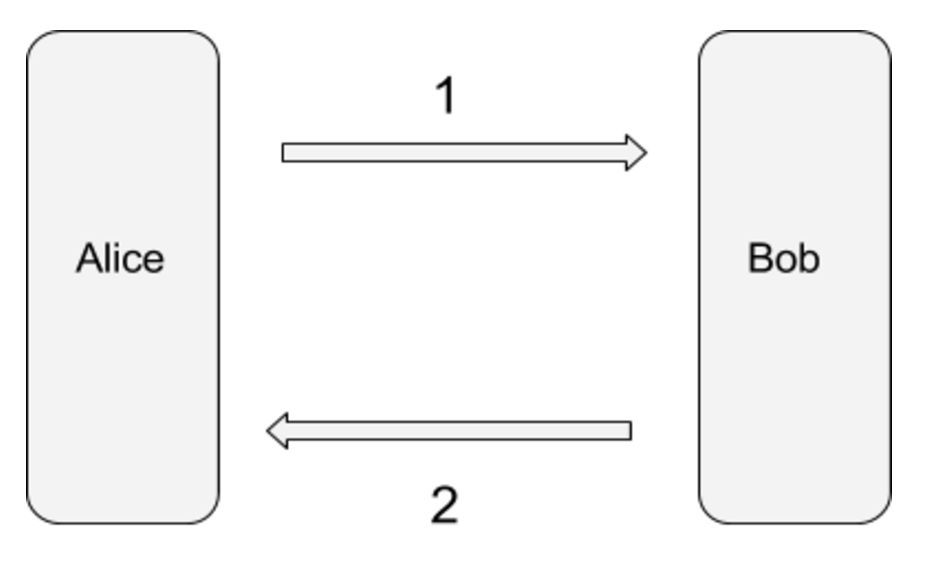
\includegraphics[width=0.5\linewidth]{protocol.png}}
\end{figure}

\textbf{1:} Alice generates a random session key $K_{AB}$ and a nonce $R1$. Alice uses her private key $A^-$ to sign a message consisting of $K_{AB}$ and $R1$ encrypted with Bob's public key $B^+$. The signature of the message (using the standard RSA signature method of hashing the message) and the message are sent to Bob.
$$m = B^+(K_{AB}, \ R1)$$
$$A^-(m), \ m$$

\textbf{2:} Bob receives Alice's signature and message. Bob uses Alice's public key $A^+$ and an identical hashing function to verify the message is from Alice. Bob uses his private key $B^-$ to decrypt $K_{AB}$ and $R1$ from $B^+(K_{AB}, \ R1)$. Bob uses $K_{AB}$ to encrypt $R1$ and sends $K_{AB}\{R1\}$ to Alice.

Finally Alice uses $K_{AB}$ to decrypt $K_{AB}\{R1\}$ and verifies $R1$ is correct.

\textbf{Security:} Bob knows $m = B^+(K_{AB}, \ R1)$ is genuinely from Alice because Alice has signed $m$. If an adversary attempts to modify $m$ during transmission, the signature will not agree and Bob will know there is an intruder.

Alice knows Bob is authentic as well. Only someone with Bob's private key can decrypt $K_{AB}$ and $R1$ from $B^+(K_{AB}, R1)$. Alice will know there is an intruder if Bob's response message $K_{AB}\{R1\}$ doesn't agree with the $K_{AB}$ and $R1$ she generated.

\part{h} \textbf{Here $\mathbf{K_{AB}}$ is the shared secret between Alice and Bob, R1 and R2 are random nonces (random numbers used only once), and the function f is a secret key function or a hash function. The protocol of this question is vulnerable to an offline dictionary attack by Trudy impersonating as Alice. Modify this protocol appropriately to remove this vulnerability.}

\question{Question 4}

\part{a} \textbf{Chapter 12, Problem 5, page 302.}

\part{b} \textbf{Chapter 12, Problem 15, page 302-303.}

\question{Question 5}

\part{a} \textbf{Let us plot the observed clock offset, in microseconds, on the y-axis and the time since the start of the finger printing measurements, in seconds, at the fingerprinter, on the x-axis. Let (6, 60) and (8, 85) be two points at times 6s and 8s, where the clock offset is observed by the fingerprinter to be 60 and 85, respectively. Estimate the clock skew of the fingerprintee from these two points. You can assume that the network delays are negligible.} 

\part{b} \textbf{Why is it not easy to fabricate clock skews of access points?}

\part{c} \textbf{Could ambient conditions change the clock skew-based fingerprints? Explain briefly. Describe one approach to deal with changes in ambient temperature.}

\part{d} \textbf{Suppose that a manufacturing plant of} \textit{linksys} \textbf{access points can produce $\mathbf{10^6}$ unique clock skew fingerprints. How many access points manufactured at this plant do you need to examine to find two that have the same fingerprint with a very high probability? After knowing this number, would you feel confident using the fingerprint method to detect unauthorized access points? Explain briefly.}

\end{document}